%%%%%%%%%%%%%%%%%%%%%%%%%%%%%%%%%%%%
% This is the template for submission to MICRO 2016
% The cls file is a modified from  'sig-alternate.cls'
%%%%%%%%%%%%%%%%%%%%%%%%%%%%%%%%%%%%

\documentclass{sig-alternate}

\newcommand{\ignore}[1]{}
\usepackage{fancyhdr}
\usepackage[normalem]{ulem}
\usepackage[hyphens]{url}
%\usepackage{hyperref}

%%%% ADDED BY GIL %%%%
\usepackage{listings}
\lstset{
    frame=single,
    breaklines=true,
    postbreak=\raisebox{0ex}[0ex][0ex]{\ensuremath{\color{black}\hookrightarrow\space}}
}

\usepackage[caption=false]{subfig}
\usepackage{array}
\newcolumntype{M}[1]{>{\centering\arraybackslash}m{#1}}
\usepackage{multirow}

\usepackage{xcolor}
\newcommand\todo[1]{\textcolor{red}{#1}}

\captionsetup[subfigure]{subrefformat=simple,labelformat=simple,listofformat=subsimple}
\renewcommand\thesubfigure{(\alph{subfigure})}

%%%%%%%%%%%---SETME-----%%%%%%%%%%%%%
\newcommand{\microsubmissionnumber}{}
%%%%%%%%%%%%%%%%%%%%%%%%%%%%%%%%%%%%

\fancypagestyle{firstpage}{
  \fancyhf{}
\setlength{\headheight}{50pt}
\renewcommand{\headrulewidth}{0pt}
  \fancyhead[C]{\normalsize{047006 - Heterogeneous Computing - Final Project
      \textbf{\microsubmissionnumber}}} 
  \pagenumbering{arabic}
}  

%%%%%%%%%%%---SETME-----%%%%%%%%%%%%%
\title{Object Detection with Jetson TX1:\\Challenges and Insights} 
%%%%%%%%%%%%%%%%%%%%%%%%%%%%%%%%%%%%

\author{
  {
  Oron Port\hspace{10 mm}
  Gil Shomron}\\[0mm]
  \{soronpo, gilsho\}@tx.technion.ac.il\\[0mm]
  Electrical Engineering\\[0mm]
  Technion --- Israel Institute of Technology
}

\begin{document}
\maketitle
\thispagestyle{firstpage}
\pagestyle{plain}



%%%%%% -- PAPER CONTENT STARTS-- %%%%%%%%

\begin{abstract}

In this short paper we explore the execution of two object detection algorithms --- \textit{Single Shot MultiBox Detector} and \textit{You Only Look Once} --- on NVIDIA Tegra TX1. We present the performance results of both algorithm, profile and explain their behavior, share installation and execution tips, and conclude with the challenges and insights of optimizing such algorithms on such platform.

\end{abstract}



%###############################################################################
%%%%%%%%%%%%%%%%%%%%%%%%%%%%%%%%%%%%%%%%%%%%%%%%%%%%%%%%%%%%%%%%%%%%%%%%
\section{Introduction}
\label{sec:intro}
%%%%%%%%%%%%%%%%%%%%%%%%%%%%%%%%%%%%%%%%%%%%%%%%%%%%%%%%%%%%%%%%%%%%%%%%

Object detection is a major rule in many different devices, from mobile phones, cameras, and IoT devices, to drones, and autonomous cars. With the aid of machine learning, detecting an object also involves its classification, as shown in Figure \ref{fig:detection_example}.

Object detection algorithms work best on GPUs. GPUs are implemented with a large number of cores (\textit{streaming multiprocessors} (SMs)), therefore the high parallelism enables algorithms, such as object detection and machines learning, to run faster than on a CPU.

With increasing demand for low-energy modules, NVIDIA manufactures an embedded platform called Jetson. We have received the Jetson TX1 to explore the performance of different object detection algorithms. NVIDIA's Jetson TX1 is an embedded system-on-module (SoM) with quad-core ARM Cortex-A57, 4GB LPDDR4 and integrated 256-core Maxwell GPU. It is useful for deploying computer vision and deep learning in 10 watts of power.

In this paper we will discuss and analyze the performance of two algorithms: (1) \textit{Single Shot MultiBox Detector} (SSD) \cite{liu2016ssd}, as implemented with Caffe, and (2) \textit{You Only Look Once} (YOLO) \cite{redmon2016you}.

The remainder of this paper is organized as follows: Section \ref{sec:results} presents SSD and YOLO performance on Tegra TX1; Section \ref{sec:profiling} analyzes the algorithms execution using NVIDIA Visual Profiler; Section \ref{sec:installation} shares installation and execution tips we have gathered along the way, and we conclude in Section \ref{sec:conclusion}.

\begin{figure}[t]
	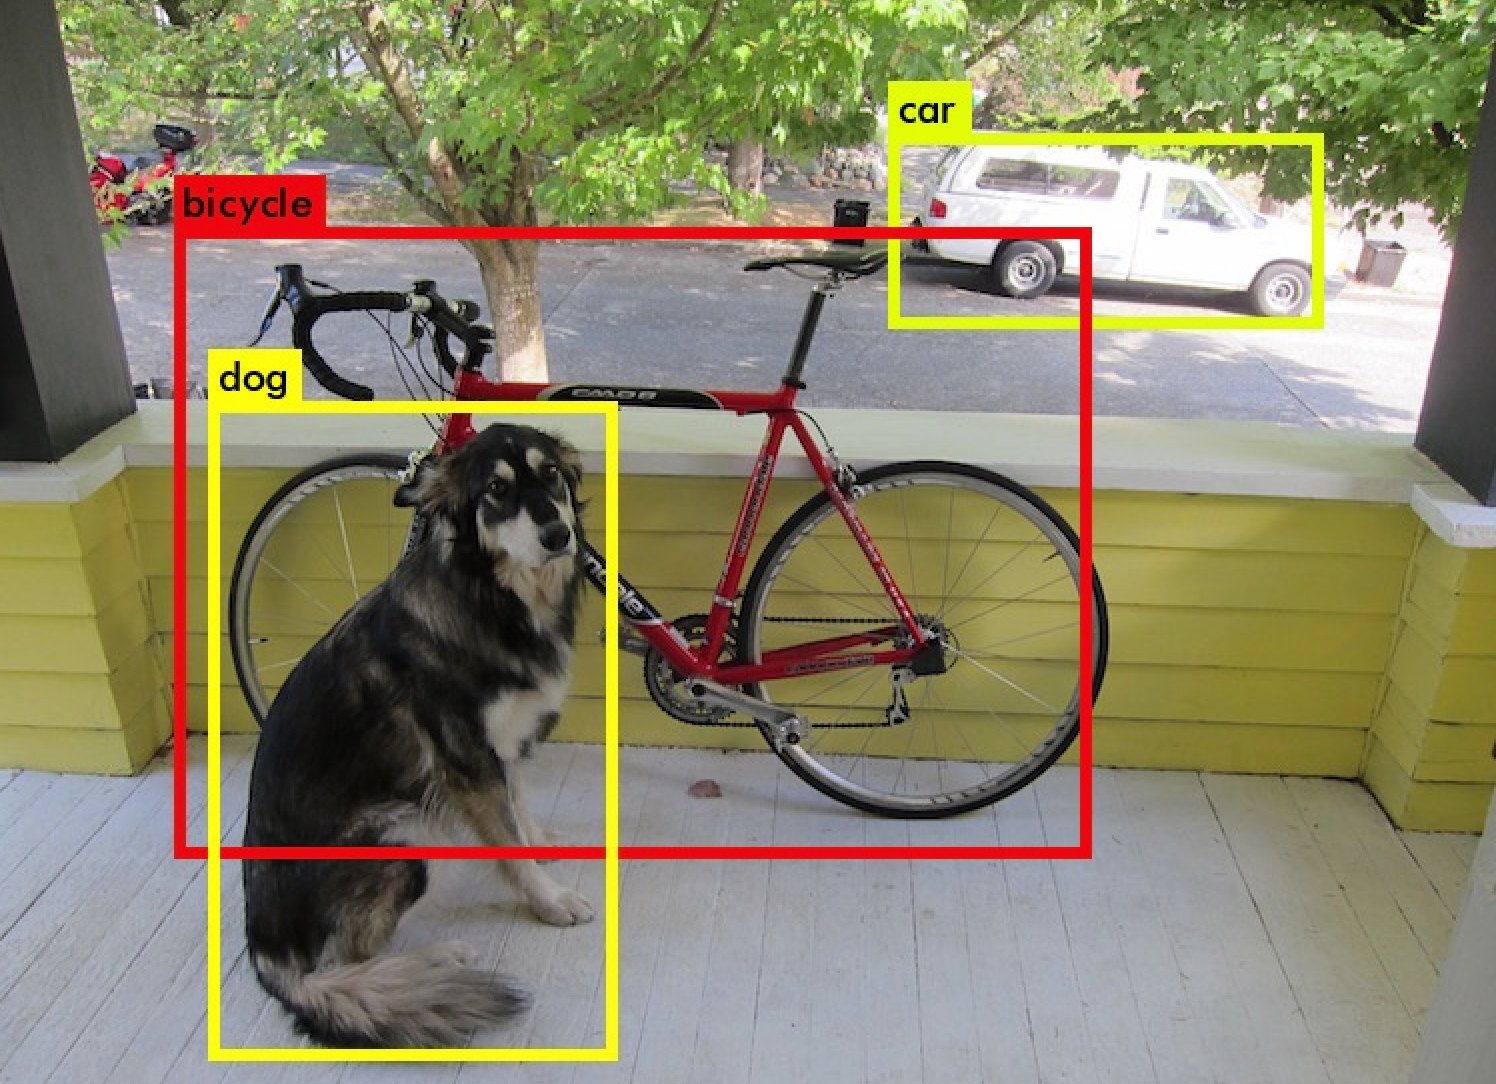
\includegraphics[width=0.48\textwidth]{./imgs/detection_example.png}
	\caption{Object detection example using YOLO}
	\label{fig:detection_example}
\end{figure}

%%%%%%%%%%%%%%%%%%%%%%%%%%%%%%%%%%%%%%%%%%%%%%%%%%%%%%%%%%%%%%%%%%%%%%%%
\section{Results} 
\label{sec:results}
%%%%%%%%%%%%%%%%%%%%%%%%%%%%%%%%%%%%%%%%%%%%%%%%%%%%%%%%%%%%%%%%%%%%%%%%

To compare SSD performance against YOLO performance on Jetson TX1, we first measured their performance on images files that reside in storage. We profiled both algorithms while they analyze 600 images from MSCOCO dataset \cite{mscoco}. The measured time is the actual kernel execution time, i.e., we do not take into consideration the CPU overheads between kernels. We made three comparison: when both algorithms run on (1) CPU, (2) GPU without cuDNN, and (3) GPU with cuDNN\footnotemark.

\footnotetext{The NVIDIA CUDA Deep Neural Network library (cuDNN) is a GPU-accelerated library of primitives for deep neural networks. cuDNN provides highly tuned implementations for standard routines such as forward and backward convolution, pooling, normalization, and activation layers.}

Figure \ref{fig:t_exec} shows the execution time of both SSD and YOLO for each of the configurations described above.
Not surprisingly, running object detection algorithms on a CPU is not as efficient as running them on a GPU. The GPU built-in parallelism is advantageous for such algorithms. The CPU performance is in order of magnitude worse than its GPU counterpart. 

The variation in the execution time when running with and without cuDNN is due to different implementations. YOLO without cuDNN performs better than with cuDNN. On the other hand, SSD with cuDNN performs better than without cuDNN.

SSD and YOLO performance is almost identical when compiled with cuDNN. It is interesting, since SSD claims to have better performance than YOLO \cite{liu2016ssd}. SSD was benchmarked with NVIDIA Titan X, which has a newer microarchitecture (Pascal vs. Maxwell), 14x more CUDA cores (3584 vs. 256), greater capacity faster memory (12GB GDDR5X vs. 4GB shared LPDDR4), and higher frequency. When system resources are scarce, the performance gains achieved by the algorithm are insignificant, therefore we do not see any major performance advantage towards SSD.

\begin{figure}[h]
	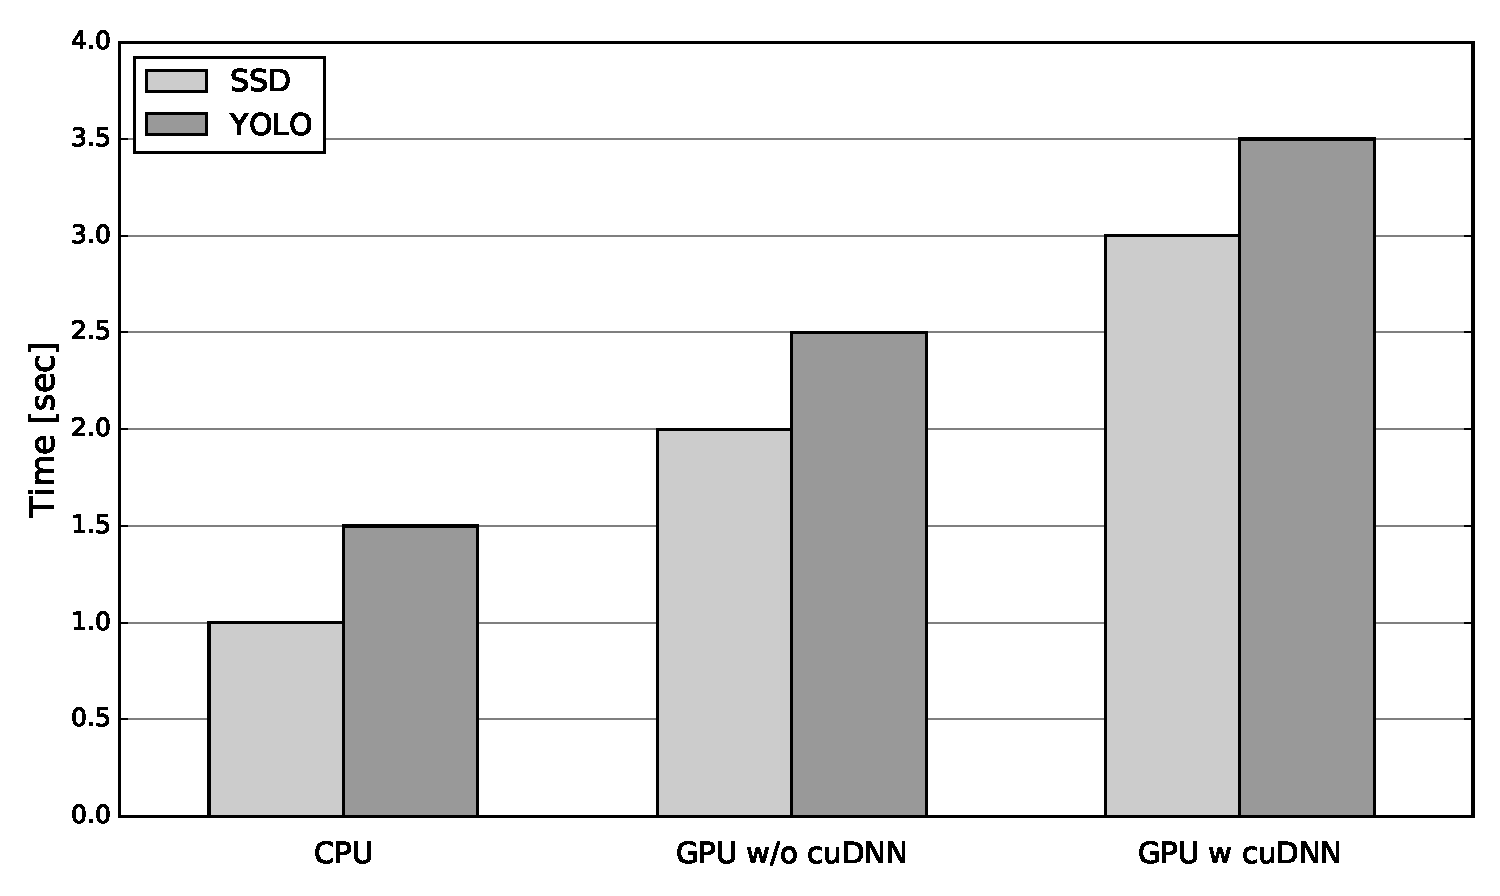
\includegraphics[width=0.48\textwidth]{./imgs/t_exec.pdf}
	\caption{Comparison of SSD and YOLO performance in different modes; CPU execution time is in order of magnitude worse than the GPU execution time}
	\label{fig:t_exec}
\end{figure}

SSD and YOLO are also packed with a web-camera demo. The original FPS readings used in the demo code are wrong, since they are based on the CPU execution time on the on the GPU execution time, therefore, the original, incorrect readings, are higher. After fixing the source code, we have measured 3.8FPS when using SSD and 4.7FPS when using YOLO. We ran the demo when both SSD and YOLO are compiled with cuDNN, and after running the \textit{jetson\_clocks.sh} script (see Section \ref{sec:installation}).

YOLO 4.7FPS fits the 200msec measurement shown in Figure \ref{fig:t_exec} ($200msec [sec/frame] = 5[frame/sec]$). The slightly lower FPS measured is due to the software overheads (e.g., fetching the images, displaying them, and drawing detection bounds).

SSD web-camera FPS is lower since the code that runs it is synchronous, meaning after an image was acquired from the web-camera it is inserted to the the neural network. YOLO web-camera demo, on the other hand, is implemented asynchronously with a double buffer, meaning that while an image is analyzed in the neural network, an image is acquired. Consequently, the acquiring time is saved. 

\begin{figure}[h]
	\subfloat[SSD: 3.8FPS]{
		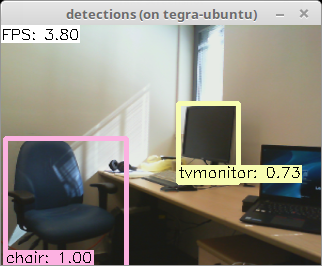
\includegraphics[width=0.23\textwidth]{./imgs/ssd_38fps.png}
		\label{fig:cam:ssd}
	}
	\subfloat[YOLO: 4.7FPS]{
		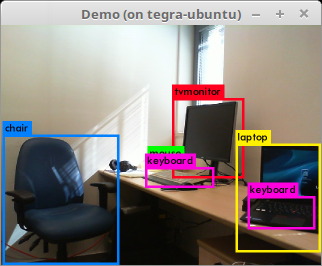
\includegraphics[width=0.23\textwidth]{./imgs/yolo_47fps.png}
		\label{fig:cam:yolo}
	}
	\caption{Object detection with SSD and YOLO using the the web-camera demo}
	\label{fig:cam}
\end{figure}
%%%%%%%%%%%%%%%%%%%%%%%%%%%%%%%%%%%%%%%%%%%%%%%%%%%%%%%%%%%%%%%%%%%%%%%%
\section{Profiling}
\label{sec:profiling}
%%%%%%%%%%%%%%%%%%%%%%%%%%%%%%%%%%%%%%%%%%%%%%%%%%%%%%%%%%%%%%%%%%%%%%%%

\begin{figure*}[t]
  \begin{center}
    \subfloat[The out on SSD (identical for YOLO): initialization phase, followed by serial object detection of images]{
      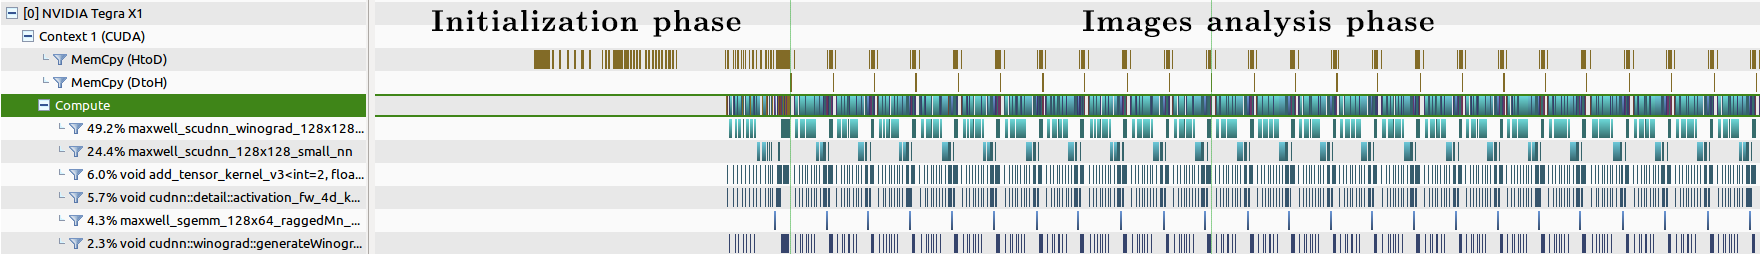
\includegraphics[width=1\textwidth]{./imgs/ssd-10frames.png}
      \label{fig:profile:ssd_full}
    } \\
    \subfloat[Zoom in on SSD: single image object detection]{
      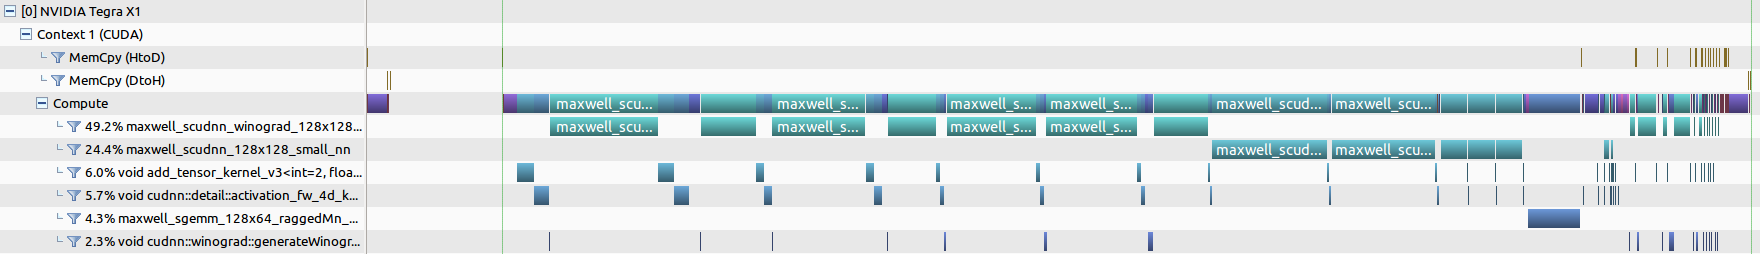
\includegraphics[width=1\textwidth]{./imgs/ssd-1frame.png}
      \label{fig:profile:ssd}
    } \\
    \subfloat[Zoom in on YOLO: single image object detection]{
      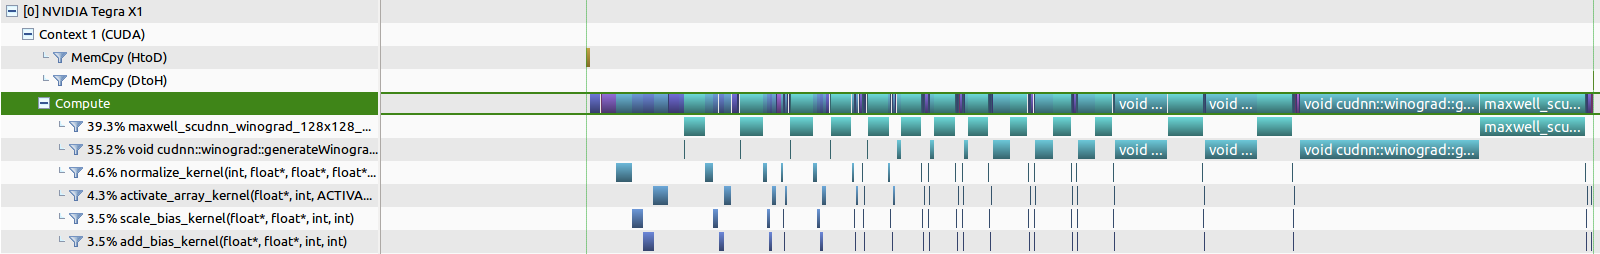
\includegraphics[width=1\textwidth]{./imgs/yolo-1frame.png}
      \label{fig:profile:yolo}
    }
    \caption{Profiling object detection on a batch of images with GPU and cuDNN on Jetson TX1, using NVIDIA Visual Profiler}
    \label{fig:profile}
  \end{center}
\end{figure*}

Figure \ref{fig:profile} shows the profiling output of object detection of a single image, using SSD and YOLO. Profiling was done using NVIDIA Visual Profiler.

One of Jetson's strengths is that its CPU and GPU share the same memory. Therefore, host-to-device (HtoD) and device-to-host (DtoH) copies can be optimized to zero-copy \cite{tegrazerocopy}. Zero-copy will have no effect on SSD and YOLO, since memory copies are not frequent, therefore, there is no speedup potential. In addition, there are no overlapping opportunities between HtoD, DtoH, and the compute kernels, since there are almost no memory copies.

In terms of compute intensity, both algorithms use 75\% of their compute time in cuDNN kernels. There is no parallelism between kernels. SSD and YOLO fetch and analyze each image in serial, so theoretically, one can analyze a couple of images in parallel. However, Jetson TX1 has only 2 SMs, with 128 CUDA cores each, therefore, adding additional threads to the system, or running two or more object detection processes in parallel, achieves no performance gains. Since SSD is implemented in Caffe as a series of layers, a possible solution may be to combine layers and avoid unwanted syncing that prevent kernel concurrency.

As can be seen from the profiling output, the dominant computation kernels belong to the cuDNN library. Both SSD and Yolo use cuDNN computations more than 70\% of the total computation time. This implementation is given, and cannot be changed by the user of the library. Therefore, the computation time cannot be improved significantly.

A major difference between SSD and Yolo, is number of memory transfers per frame. While Yolo has a single DtoH transfer and a single HtoD, SDD has 32 DtoH transfers and 2 HtoD transfers. Most of the SSD DtoH transfers are 16 bytes in size; very small and inefficient transfers. We did not manage to isolate the SSD Caffe layers that cause this issue.  




%%%%%%%%%%%%%%%%%%%%%%%%%%%%%%%%%%%%%%%%%%%%%%%%%%%%%%%%%%%%%%%%%%%%%%%%
\section{Installation and Execution}
\label{sec:installation}
%%%%%%%%%%%%%%%%%%%%%%%%%%%%%%%%%%%%%%%%%%%%%%%%%%%%%%%%%%%%%%%%%%%%%%%%
Some aspects of the Jetson installation process are not trivial. In this section, we share some installation tips, gathered during this project. It is our hope that these tips will help others to avoid our obstacles.

\subsection{Jetson TX1 Hardware Kit}
The kit includes most of the hardware required, but is \textbf{missing} the following:
\begin{itemize}
\setlength\itemsep{0.1em}
\item Power Cable -- Must
\item Network Cable -- Must
\item External USB Web Camera -- Must (if camera is required for the application)
\item USB Keyboard -- Optional
\item USB Mouse -- Optional
\item HDMI Cable -- Optional (with an HDMI supported monitor)
\item USB Flash Drive -- Optional (If extra space is required)
\end{itemize}

The on-board camera is not well supported, while a simple USB web camera connected to the USB worked right out-of-the-box.

The optional components are required to debug the system. All the work can be done via SSH, but our initial system bring-up had unexpected problems. Hopefully, using the tips we layout here, others will be able to avoid this in the future.

\subsection{Jetpack SDK Installation}
Download the latest Jetpack SDK~\cite{jetpackinstall}. NVIDIA developer membership is required (registration is free).
It is best to connect the Jetson to a router and SSH to it via internal network. The initial setup requires a host computer connected via USB to the Jetson. The host \textbf{must} be an Ubuntu 14.04 machine. It is possible (and recommended) to use a Virtual Machine software with the proper image. We used Virtual Box~\cite{virtualboxinstall} with the Ubuntu 14.04.05 Trusty image~\cite{virtualboxubuntuimage}. Do not confuse with the 64-bit Ubuntu 16.04 version, which is installed on the Jetson.

The Jetpack installs an optimized OpenCV library, but of an old version. We attempted to updated to a newer version, but had too many complication. It is our recommendation to leave the installed version as is.

The Jetson has very little installation space (\~14GB). It is possible to remove the installation files to free space after the installation. In any case, it is recommended to have an EXT3/EXT4 formatted USB flash drive available (FAT/NTFS formatted drives do not work as well). 

\subsection{Caffe Installation}

The SSD Caffe \cite{caffessd} is a fork of the Caffe library \cite{caffeoriginal}. When cloning/downloading the project it is required to use the \textit{ssd} branch.

During Caffe compilation we suffered many system restarts. We figured out that the CPU fan is not turned-on by default, which causes the system to heat-up. \textbf{The fan must be turned on!} To turn the fan, the following command must be executed in sudo:
\begin{lstlisting} 
echo 255 > /sys/kernel/debug/tegra_fan/target_pwm
\end{lstlisting}
However, calling sudo directly with the command does not work. Create a shell script that includes the command, and use \textit{sudo} to call the script instead. We recommend to have an alias handy in your \textit{.bashrc} file. For example:
\begin{lstlisting} 
alias start-fan="sudo ~/start-fan.sh"
\end{lstlisting}
Call start-fan for every system restart.

\textbf{Makefile.config}. 
When compiling the Caffe library, you create and modify 
To use cuDNN acceleration modify the flag:
\begin{lstlisting} 
USE_CUDNN := 1
\end{lstlisting}

Tegra X1 has CUDA capability 5.3, therefore append to \textit{CUDA\_ARCH}: 
\begin{lstlisting} 
CUDA_ARCH := -gencode arch=compute_53, code=sm_53
\end{lstlisting}

HDF5 directories should be added to \textit{INCLUDE\_DIRS} and \textit{LIBRARY\_DIRS}:
\begin{lstlisting} 
INCLUDE_DIRS := $(PYTHON_INCLUDE) /usr/local/include /usr/include/hdf5/serial
LIBRARY_DIRS := $(PYTHON_LIB) /usr/local/lib /usr/lib/aarch64-linux-gnu/serial
\end{lstlisting}

\textbf{Makefile}.
HDF5 libraries need to be added to the Makefile also:
\begin{lstlisting} 
LIBRARIES += glog gflags protobuf boost_system boost_filesystem m hdf5_serial_hl hdf5_serial
\end{lstlisting}

\textbf{Python and Caffe paths}.
Caffe also has Python libraries. Running Python scripts can fail due to unset Python path. By adding the following to ~/.bashrc :
\begin{lstlisting} 
export CAFFE_ROOT=$HOME/caffe
export PYTHONPATH=$CAFFE_ROOT/python
\end{lstlisting}
where \textit{\$CAFFE\_ROOT} is the Caffe home directory, we managed to fix the issues. 

\textbf{Compiling}.
Make sure to use '-j4' flag for a faster make. For python programs 'make py' must also be executed.
\begin{lstlisting} 
make -j4
make py
\end{lstlisting}

\textbf{Example Images and Pretrained models}.
We used the pretrained models and example images available on the Caffe site.

\textbf{Web Camera}.
Jetson TX1 on-board CSI camera does not work straightaway. Alternatively, plugging a dedicated web-camera almost does. To run Caffe SSD web-camera demo, we run the following from the Caffe root directory:
\begin{lstlisting} 
LD_PRELOAD=/usr/lib/aarch64-linux-gnu/libv4l/v4l2convert.so python examples/ssd/ssd_pascal_webcam.py
\end{lstlisting}

Smaller resolution with faster FPS can be obtained by changing the display scale 
in ssd\_pascal\_webcam.py:
\begin{lstlisting} 
# Scale the image size for display.
scale = 0.5
\end{lstlisting}

Running the demo for a limited time can be done by modifying the number of iterations (frames) in ssd-\_pascal\_webcam.py:
\begin{lstlisting} 
# Set the number of test iterations to the maximum integer number.
test_iter = 30 
\end{lstlisting}

\textbf{Fixing the FPS indication}. We noticed that the FPS indication is wrong. To fix this issue we modified the bbox\_util.cpp file. The original time measurement used the \textit{clock()} function which measures CPU time, while most computation is done on the GPU. To get the real time between frames we used \textit{clock\_gettime()} instead. Full implementation can be viewed in our repository.

\textbf{Performance Tuning.}
The new Tegra Linux driver package releases include \textit{jetson\_clocks.sh} script, this is able to maximize performance by disabling DVFS, CPU idle, and CPU quit \cite{tegradriverpack242}. To toggle performance:
\begin{lstlisting} 
sudo ./jetson_clocks.sh
\end{lstlisting}
This script also turns on the fan. We recommend reading the manual first.

\subsection{YOLO Installation}
The installation of yolo is straightforward. Notice that the running \textit{tiny-yolo} to achieve higher FPS, rendered too many false detections.
We modified the detector.c file to read a list of images, similarly to the Caffe ssd\_detect functionality. The demo.c file can be modified to set the display resolution to match the Caffe display resolution for proper comparison.

Notice that \textit{detector.c} does not measure the detection time correctly (same bug as in Caffe), but the \textit{demo.c} FPS counter is properly implemented.

\subsection{Running the NVIDIA Profiler}
Using the tool is fairly simple. Note that it cannot be used to profile the web-cam demo applications since they open a GUI, and the profiler does not connect an SSH with \textit{X}. Additionally, the tool enables setting a profiling timeout, which can be used to partially profile a long running test. 

%%%%%%%%%%%%%%%%%%%%%%%%%%%%%%%%%%%%%%%%%%%%%%%%%%%%%%%%%%%%%%%%%%%%%%%%
\section{Conclusion}
\label{sec:conclusion}
%%%%%%%%%%%%%%%%%%%%%%%%%%%%%%%%%%%%%%%%%%%%%%%%%%%%%%%%%%%%%%%%%%%%%%%%

SSD and YOLO are not I/O intensive but compute intensive. Since 75\% of execution time the algorithms runs cuDNN, which is a well optimized library provided by NVIDIA, we think that in this project time frame it is not possible to optimize SSD or YOLO any further. Even if one will optimize the remaining 25\%, the 10FPS goal will not be achieved (Amdahl's law).

It is possible to increase the performance of the above algorithms on a Jetson TX1 by modifying the algorithms, probably on the expense of accuracy. For example, Tiny YOLO is a faster version of YOLO. It exhibits 4x speedup over the regular YOLO (according to their website). The trade-off is unbearable error rate. Unfortunately, we did not find a model that fits in between.

A simple solution to scale performance is scaling the number of Jetson boards, it would be interesting to see whether performance increase linearly with the increase of the number of Jetsons. It will be also interesting to measure the power consumption of such architecture versus its performance.

%###############################################################################


%%%%%%% -- PAPER CONTENT ENDS -- %%%%%%%%


%%%%%%%%% -- BIB STYLE AND FILE -- %%%%%%%%
\bibliographystyle{ieeetr}
\bibliography{jetson_obj_detect}
%%%%%%%%%%%%%%%%%%%%%%%%%%%%%%%%%%%%

\end{document}
